\begin{figure}
    \centering
    \resizebox{0.75\linewidth}{!}{
    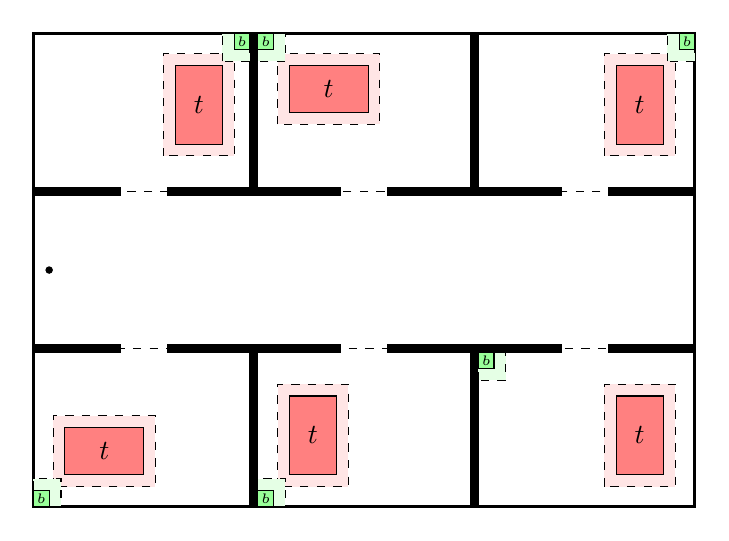
\begin{tikzpicture}
    
        % Boundary
        \draw[very thick, fill = white] (0, 0) rectangle (8.4, 6);
        \draw[dashed] (0,2) -- (8.4,2) -- (8.4, 4) -- (0,4);
        
        % Vertical walls
        \filldraw (2.75, 0) rectangle (2.85, 2.05);
        \filldraw (2.75, 3.95) rectangle (2.85, 6);
        \filldraw (5.55, 0) rectangle (5.65, 2.05);
        \filldraw (5.55, 3.95) rectangle (5.65, 6);
        
        % Horizontal walls
        \filldraw (0, 1.95) rectangle (1.1, 2.05);
    	\filldraw (0, 3.95) rectangle (1.1, 4.05);
        \filldraw (1.7, 1.95) rectangle (3.9, 2.05);
    	\filldraw (1.7, 3.95) rectangle (3.9, 4.05);
        \filldraw (4.5, 1.95) rectangle (6.7, 2.05);
    	\filldraw (4.5, 3.95) rectangle (6.7, 4.05);
        \filldraw (7.3, 1.95) rectangle (8.4, 2.05);
        \filldraw (7.3, 3.95) rectangle (8.4, 4.05);
        
    	% Table label lines
    	\filldraw[dashed, fill = red!10!white] (0.25,0.25) rectangle (1.55,1.15); % r1
    	\filldraw[dashed, fill = red!10!white] (1.65,4.45) rectangle (2.55,5.75); %r2
    	\filldraw[dashed, fill = red!10!white] (3.1,0.25) rectangle (4,1.55); % r3
    	\filldraw[dashed, fill = red!10!white] (3.1,4.85) rectangle (4.4,5.75); %r4
    	\filldraw[dashed, fill = red!10!white] (7.25,0.25) rectangle (8.15,1.55); % r5
    	\filldraw[dashed, fill = red!10!white] (7.25,4.45) rectangle (8.15,5.75); %r6
    	
    	% Bin label lines
    	\filldraw[dashed, fill = green!10!white] (0,0) rectangle (0.35,0.35); % r1
    	\filldraw[dashed, fill = green!10!white] (2.4,5.65) rectangle (2.75,6); % r2
    	\filldraw[dashed, fill = green!10!white] (2.85,0) rectangle (3.2,0.35); % r3
    	\filldraw[dashed, fill = green!10!white] (2.85,5.65) rectangle (3.2,6); % r4
    	\filldraw[dashed, fill = green!10!white] (5.65,1.6) rectangle (6,1.95); % r5
    	\filldraw[dashed, fill = green!10!white] (8.05,5.65) rectangle (8.4,6); % r6
    	
    	% Bins
    	\filldraw[fill = green!40!white] (0, 0) rectangle (0.2, 0.2) node[midway] {\tiny $b$}; % r1
    	\filldraw[fill = green!40!white] (2.55, 5.8) rectangle (2.75, 6) node[midway] {\tiny $b$}; % r2
    	\filldraw[fill = green!40!white] (2.85, 0) rectangle (3.05, 0.2) node[midway] {\tiny $b$}; % r3
    	\filldraw[fill = green!40!white] (2.85, 5.8) rectangle (3.05, 6) node[midway] {\tiny $b$}; % r4
    	\filldraw[fill = green!40!white] (5.65, 1.75) rectangle (5.85, 1.95) node[midway] {\tiny $b$}; % r5
    	\filldraw[fill = green!40!white] (8.2, 5.8) rectangle (8.4, 6) node[midway] {\tiny $b$}; % r6
    	
    	% Tables
    	\filldraw[fill = red!50!white] (0.4, 0.4) rectangle (1.4, 1) node[midway] {$t$}; % r1
    	\filldraw[fill = red!50!white] (1.8, 4.6) rectangle (2.4, 5.6) node[midway] {$t$}; % r2
    	\filldraw[fill = red!50!white] (3.25, 0.4) rectangle (3.85, 1.4) node[midway] {$t$}; % r3
    	\filldraw[fill = red!50!white] (3.25, 5) rectangle (4.25, 5.6) node[midway] {$t$}; % r4
    	\filldraw[fill = red!50!white] (7.4, 0.4) rectangle (8.0, 1.4) node[midway] {$t$}; % r5
    	\filldraw[fill = red!50!white] (7.4, 4.6) rectangle (8.0, 5.6) node[midway] {$t$}; % r6
    	
    	\filldraw[black] (0.2, 3) circle (0.4mm);
    \end{tikzpicture}
    }
    \caption{Example of an office-like environment used in the case study. Black solid lines represent walls. There are six rooms, each labeled with one atomic proposition $r_i$, for $i \in [1,6]$, and a hallway labeled $h$. Each room contains a table (red) and a bin (green), labeled $t$ and $b$, respectively. The labels of tables and bins hold true within the corresponding dashed and shaded areas surrounding it. The initial position of the robot is marked with a black dot on the left side of the hallway.}
    \label{fig:example}
\end{figure}

